\documentclass[12pt, a4paper]{article}

% ── Shared preamble (src/lecturenotes.sty) ────────────────────────────────────
%   Packages, colors, boxes, \sol/\soleq and math macros all live in
%   src/*.sty. \input@path points LaTeX two folders up to find them.
\makeatletter
\def\input@path{{../../}}
\makeatother
\usepackage{lecturenotes}

% ── Local macros ──────────────────────────────────────────────────────────────
\providecommand{\bZ}{\mathbf{Z}}
\providecommand{\bH}{\mathbf{H}}
\providecommand{\bdelta}{\boldsymbol{\delta}}

% ── Local TikZ styles ─────────────────────────────────────────────────────────
\usetikzlibrary{decorations.pathreplacing}
\tikzset{
  layerlabel/.style={font=\small\itshape, gray},
  brace/.style={decorate, decoration={brace, amplitude=4pt}, thick, gray},
  window/.style={draw=orange!80!black, line width=1.6pt},
  outcell/.style={draw=mainblue, line width=1.6pt},
  opbox/.style={draw=orange!70!black, fill=notebg, thick, rounded corners=4pt,
      minimum height=0.9cm, minimum width=1.9cm, font=\small, align=center},
}

% \drawgrid{<shift>}{<fill>}{<rows>} — grid of unit cells with values,
%   rows given as {a,b,c},{d,e,f},... ; row 1 at the top.
\newcommand{\drawgrid}[3]{%
  \begin{scope}[shift={#1}]
    \foreach \row [count=\r] in {#3} {
        \foreach \v [count=\c] in \row {
            \draw[gray!70, fill=#2] (\c-1,-\r+1) rectangle ++(1,-1);
            \node[font=\small] at (\c-0.5,-\r+0.5) {$\v$};
          }
      }
  \end{scope}%
}

% \cuboid{<x>}{<depth: channels>}{<height: spatial>}{<color>}{<label>}
%   pseudo-3D block for a (C, H, W) tensor, centred vertically on y = 0
\newcommand{\cuboid}[5]{%
  \pgfmathsetmacro{\off}{#3*0.3}
  \filldraw[fill=#4!20, draw=#4!80!black] (#1,-#3/2) rectangle ++(#2,#3);
  \filldraw[fill=#4!35, draw=#4!80!black]
  (#1,#3/2) -- ++(\off,\off) -- ++(#2,0) -- ++(-\off,-\off) -- cycle;
  \filldraw[fill=#4!50, draw=#4!80!black]
  (#1+#2,-#3/2) -- ++(\off,\off) -- ++(0,#3) -- ++(-\off,-\off) -- cycle;
  \node[below, font=\scriptsize, align=center] at (#1+#2/2,-1.75) {#5};
}

% ── Document ──────────────────────────────────────────────────────────────────
\begin{document}

\begin{center}
  {\LARGE \textbf{Section 4.1: Convolutional Neural Networks}} \\[0.3em]
  {\large\itshape From Convolution to a Complete CNN} \\[0.5em]
  {\large AI-IM Class --- Lecture Notes}%
  \ifstudentmode
    \quad {\normalsize\color{gray}[Student Copy]}%
  \fi
\end{center}

\vspace{1em}
\hrule
\vspace{1.5em}

In Section 3.4 we built a complete classifier: a stack of fully connected
layers, a softmax output and the cross-entropy loss. In this chapter the
input is an \textbf{image}, and we replace the fully connected layers at the
front of the network by \textbf{convolutional} layers. In this section we
\begin{itemize}[nosep]
  \item see why an MLP is a poor fit for images,
  \item define convolution in one and two dimensions, with \emph{padding},
        \emph{stride} and \emph{channels},
  \item add activation and \emph{pooling} and assemble a complete CNN, and
  \item see how gradients flow back through a CNN layer.
\end{itemize}

% ══════════════════════════════════════════════════════════════════════════════
\section{Why Convolutional Networks?}
\label{sec:why}

\paragraph{Images as data.}
\begin{itemize}[nosep]
  \item A grayscale image is a grid of pixel values; a colour image stores
        three such grids (red, green, blue), called \textbf{channels}.
  \item An image is a tensor of shape $(C, H, W)$: channels, height, width.
        In PyTorch a mini-batch of $N$ images has shape $(N, C, H, W)$.
\end{itemize}

\begin{figure}[H]
  \centering
  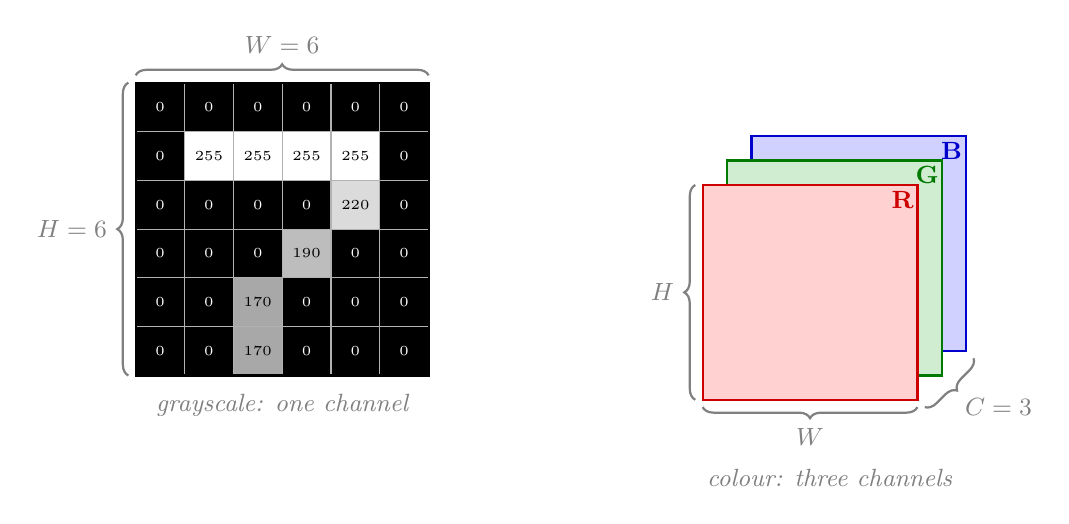
\begin{tikzpicture}[x=0.62cm, y=0.62cm]
    \foreach \row [count=\r] in {
        {0,0,0,0,0,0},
        {0,255,255,255,255,0},
        {0,0,0,0,220,0},
        {0,0,0,190,0,0},
        {0,0,170,0,0,0},
        {0,0,170,0,0,0}} {
        \foreach \v [count=\c] in \row {
          \pgfmathtruncatemacro{\p}{\v/255*100}
          \pgfmathtruncatemacro{\dark}{\v<128}
          \fill[white!\p!black] (\c-1, -\r+1) rectangle ++(1,-1);
          \ifnum\dark=1
            \node[font=\tiny, white] at (\c-0.5, -\r+0.5) {\v};
          \else
            \node[font=\tiny, black] at (\c-0.5, -\r+0.5) {\v};
          \fi
        }
      }
    \draw[gray!60, step=1] (0,0) grid (6,-6);
    \draw[thick] (0,0) rectangle (6,-6);
    \draw[brace] (0,0.15) -- node[above=4pt, font=\small] {$W = 6$} (6,0.15);
    \draw[brace] (-0.15,-6) -- node[left=4pt, font=\small] {$H = 6$} (-0.15,0);
    \node[layerlabel] at (3,-6.6) {grayscale: one channel};

    % ── colour image: three stacked channels ─────────────────────────────────
    \begin{scope}[xshift=7.2cm, yshift=-1.3cm]
      \foreach \col/\lbl/\s in {blue/B/2, green!60!black/G/1, red/R/0} {
          \filldraw[fill=\col!18, draw=\col!80!black, thick]
          (0.5*\s, 0.5*\s) rectangle ++(4.4, -4.4);
          \node[font=\small\bfseries, text=\col!80!black]
          at (0.5*\s+4.1, 0.5*\s-0.3) {\lbl};
        }
      \draw[brace] (4.4,-4.55) -- node[below=4pt, font=\small] {$W$} (0,-4.55);
      \draw[brace] (-0.15,-4.4) -- node[left=4pt, font=\small] {$H$} (-0.15,0);
      \draw[brace] (5.55,-3.55) -- node[below right=2pt, font=\small] {$C = 3$}
      (4.55,-4.55);
      \node[layerlabel] at (2.6,-6.0) {colour: three channels};
    \end{scope}
  \end{tikzpicture}
  \caption{Left: a $6\times 6$ grayscale image of the digit ``7'' and its pixel
    values. Right: a colour image stores three such grids, one per
    \emph{channel} (red, green, blue).}
  \label{fig:image}
\end{figure}

\paragraph{Three weaknesses of an MLP on images.}
To feed an image to an MLP we must \textbf{flatten} it into one long vector.
\begin{itemize}[nosep]
  \item \textbf{Too many parameters.} Every pixel connects to every node, so
        the first layer becomes enormous for realistic image sizes.
  \item \textbf{Flattening ignores which pixels are neighbours.} Pixels that
        are next to each other in the image end up far apart in the vector,
        and the MLP has to relearn the layout from data.
  \item \textbf{A pattern learned in one place is unknown elsewhere.} A node
        that detects a feature at one position does not detect it at another,
        so the same pattern must be learned again for every position.
\end{itemize}

\paragraph{Three key ideas.}
A convolution slides one small set of weights, a \textbf{kernel} (or
\textbf{filter}), across the image and computes a weighted sum at each
position. This gives three properties (Goodfellow et al., \emph{Deep
  Learning}, Section 9.2):
\begin{itemize}[nosep]
  \item \textbf{Sparse interactions.} Each output depends only on a small
        patch of the input, its \textbf{receptive field}.
  \item \textbf{Parameter sharing.} The same kernel is reused at every
        position, so the number of weights does not depend on the image
        size.
  \item \textbf{Equivariance to translation.} Shift the input and the output
        (a \textbf{feature map}) shifts by the same amount.
\end{itemize}
Stacking convolutional layers enlarges the receptive field, so deep CNNs form
a hierarchy: edges $\to$ textures and parts $\to$ objects.

% ══════════════════════════════════════════════════════════════════════════════
\section{Convolution in One Dimension}

\paragraph{Notation.}
As in Section 3.4, bold capitals are arrays and lower-case letters are their
entries. The input is $\bX$ with entries $x_{i,j}$; the kernel is $\bW$ with
entries $w_{u,v}$; the output (pre-activation) is $\bZ$ with entries
$z_{i,j}$; $b$ is the bias. The kernel has size $k \times k$. Do not confuse
the bold kernel $\bW$ with the italic image width $W$.

\medskip
Let $\bx = (x_1, \dots, x_n)$ be an input of length $n$ and
$\bw = (w_1, \dots, w_k)$ a kernel of length $k \le n$. Place the kernel at
position $i$, multiply the overlapping entries, and add:

\begin{resultbox}
  \[
    z_i = \sum_{u=1}^{k} w_u\, x_{i+u-1} + b,
    \qquad i = 1, 2, \dots, n - k + 1.
  \]
  The output has length $n - k + 1$.
\end{resultbox}

\paragraph{Why $i + u - 1$?}
Both the input and the kernel are numbered from $1$. The window for $z_i$
starts at $x_i$, so kernel entry $w_u$ meets the input $u - 1$ places further
on: $w_1$ meets $x_i$, $w_2$ meets $x_{i+1}$, \dots, $w_k$ meets
$x_{i+k-1}$. The last window must still fit, $i + k - 1 \le n$, which is where
the output length $n - k + 1$ comes from. (With 0-based indexing, as in
Python, the formula is simply $z_i = \sum_{u} w_u\, x_{i+u} + b$.)

\begin{figure}[H]
  \centering
  \begin{tikzpicture}[x=0.9cm, y=0.9cm, >=Stealth]
    \drawgrid{(0,0)}{white}{{1,3,2,0,4}}
    \node[anchor=east, font=\small] at (-0.2,-0.5) {$\bx$};
    \draw[window] (1,0) rectangle (4,-1);

    \drawgrid{(1,-1.8)}{notebg}{{1,0,-1}}
    \node[anchor=east, font=\small] at (0.8,-2.3) {$\bw$};
    \foreach \u in {1,2,3} \draw[->, gray] (\u+0.5,-1.75) -- (\u+0.5,-1.05);

    \drawgrid{(1,-3.6)}{boxbg}{{z_1,z_2,z_3}}
    \node[anchor=east, font=\small] at (0.8,-4.1) {$\bz$};
    \draw[outcell] (2,-3.6) rectangle (3,-4.6);

    \node[font=\small, anchor=west, align=left] at (5.6,-2.1)
    {position $i = 2$:\\
      $z_2 = (1)(3) + (0)(2) + (-1)(0)$};
  \end{tikzpicture}
  \caption{One-dimensional convolution with $n = 5$ and $k = 3$ (bias $b = 0$).
    The kernel slides one step at a time; the window at position $i = 2$ is
    outlined.}
  \label{fig:conv1d}
\end{figure}

\begin{stepbox}{Exercise 1 \quad A 1-D convolution}
  Use $\bx = (1, 3, 2, 0, 4)$, $\bw = (1, 0, -1)$ and $b = 0$, as in
  Figure~\ref{fig:conv1d}.
  \begin{enumerate}[label=(\alph*), nosep]
    \item The output has length $\sol[3cm]{5 - 3 + 1 = 3}$.
    \item $z_1 = \sol[4cm]{1 - 2 = -1}$, \quad
          $z_2 = \sol[3cm]{3 - 0 = 3}$, \quad
          $z_3 = \sol[3cm]{2 - 4 = -2}$.
    \item This kernel computes $z_i = x_i - x_{i+2}$. It measures how much the
          signal $\sol[2.5cm]{\text{decreases}}$ over two steps.
  \end{enumerate}
\end{stepbox}

\begin{notebox}
  \textbf{Convolution or cross-correlation?}
  In mathematics and signal processing, \emph{convolution} flips the kernel
  before sliding it:
  $(x * w)_i = \sum_{u} x_{i-u}\, w_u$. The operation in the box above, which
  does not flip, is strictly called \textbf{cross-correlation}.
  With the flipped kernel $(-1, 0, 1)$, Exercise 1 would give
  $\bz = (1, -3, 2)$: the same numbers with opposite sign.

  In a CNN the kernel values are \emph{learned}. If the flipped version is
  better, training simply learns the flipped numbers, so the choice makes no
  difference. Deep-learning libraries, including PyTorch's
  \texttt{nn.Conv1d} and \texttt{nn.Conv2d}, compute cross-correlation and
  call it convolution. We do the same.
\end{notebox}

% ══════════════════════════════════════════════════════════════════════════════
\section{Convolution in Two Dimensions}
\label{sec:conv2d}

For an image the kernel is a small $k \times k$ grid that slides across both
rows and columns. At each position we multiply the kernel entrywise with the
$k \times k$ patch beneath it and add everything up.

\begin{resultbox}
  \[
    z_{i,j} = \sum_{u=1}^{k} \sum_{v=1}^{k} w_{u,v}\; x_{i+u-1,\; j+v-1} + b .
  \]
  For an $H \times W$ input the output is
  $(H - k + 1) \times (W - k + 1)$.
\end{resultbox}

The output is called a \textbf{feature map}: entry $z_{i,j}$ says how
strongly the pattern in the kernel is present in the patch whose top-left
corner is pixel $(i, j)$. As in one dimension, the $-1$ in the indices makes
the kernel's top-left entry $w_{1,1}$ meet that corner pixel $x_{i,j}$, and
the last window must fit inside the image, giving the output size
$(H - k + 1) \times (W - k + 1)$.

\begin{figure}[H]
  \centering
  \begin{tikzpicture}[x=0.72cm, y=0.72cm, >=Stealth]
    \drawgrid{(0,0)}{white}{{0,0,0,0,0},{0,0,0,0,0},{0,0,1,1,1},{0,0,1,1,1},{0,0,1,1,1}}
    \fill[orange!20, opacity=0.6] (0,0) rectangle (3,-3);
    \draw[window] (0,0) rectangle (3,-3);
    \node[layerlabel] at (2.5,-5.6) {input $\bX$ ($5\times5$)};

    \node[font=\Large] at (6.0,-2.5) {$\ast$};

    \drawgrid{(7,-1)}{notebg}{{-1,0,1},{-1,0,1},{-1,0,1}}
    \node[layerlabel, align=center] at (8.5,-4.9) {kernel $\bW_{\!v}$\\($3\times3$)};

    \node[font=\Large] at (11.0,-2.5) {$=$};

    \drawgrid{(12,-1)}{boxbg}{{z_{1,1},z_{1,2},z_{1,3}},{z_{2,1},z_{2,2},z_{2,3}},{z_{3,1},z_{3,2},z_{3,3}}}
    \draw[outcell] (12,-1) rectangle (13,-2);
    \node[layerlabel, align=center] at (13.5,-4.9) {feature map $\bZ$\\($3\times3$)};

    \draw[->, orange!80!black, thick] (3,0) to[bend left=20] (12.5,-0.95);
  \end{tikzpicture}
  \caption{Two-dimensional convolution. The input contains a bright square in
    its lower-right corner. The outlined $3\times3$ patch, multiplied entrywise
    by the kernel and summed, gives $z_{1,1}$. Sliding the patch one column
    right gives $z_{1,2}$, and so on.}
  \label{fig:conv2d}
\end{figure}

\begin{stepbox}{Exercise 2 \quad Detecting edges by hand}
  Use the input $\bX$ of Figure~\ref{fig:conv2d} with $b = 0$ and two
  kernels:
  \[
    \bW_{\!v} =
    \begin{pmatrix} -1 & 0 & 1 \\ -1 & 0 & 1 \\ -1 & 0 & 1 \end{pmatrix},
    \qquad
    \bW_{\!h} =
    \begin{pmatrix} -1 & -1 & -1 \\ 0 & 0 & 0 \\ 1 & 1 & 1 \end{pmatrix}.
  \]
  $\bW_{\!v}$ computes (right column of the patch) $-$ (left column);
  $\bW_{\!h}$ computes (bottom row) $-$ (top row).
  \[
    \bZ_v =
    \begin{pmatrix}
      \sol[0.6cm]{1} & \sol[0.6cm]{1} & \sol[0.6cm]{0} \\[2pt]
      \sol[0.6cm]{2} & \sol[0.6cm]{2} & \sol[0.6cm]{0} \\[2pt]
      \sol[0.6cm]{3} & \sol[0.6cm]{3} & \sol[0.6cm]{0}
    \end{pmatrix},
    \qquad
    \bZ_h =
    \begin{pmatrix}
      \sol[0.6cm]{1} & \sol[0.6cm]{2} & \sol[0.6cm]{3} \\[2pt]
      \sol[0.6cm]{1} & \sol[0.6cm]{2} & \sol[0.6cm]{3} \\[2pt]
      \sol[0.6cm]{0} & \sol[0.6cm]{0} & \sol[0.6cm]{0}
    \end{pmatrix}
  \]
  Where in the image is $\bZ_v$ largest, and why?
  \soleq[1.2cm]{\parbox{0.85\linewidth}{\raggedright Bottom-left: those
      patches contain the whole vertical edge of the square (dark on the left,
      bright on the right, in all three rows).}}
\end{stepbox}

The two kernels respond to different features of the \emph{same} image:
$\bW_{\!v}$ to the left (vertical) edge of the square, $\bW_{\!h}$ to its
top (horizontal) edge. Inside the square, where the image is flat, both are
zero.

\begin{notebox}
  \textbf{Hand-designed vs.\ learned kernels.}
  $\bW_{\!v}$ and $\bW_{\!h}$ are classical image-processing filters (the
  \emph{Prewitt} filters), designed by hand. In a CNN the nine numbers in each
  kernel are \emph{parameters}, found by gradient descent like any other
  weight. When we look at the kernels a trained CNN learned in its first
  layer, many turn out to be edge and colour detectors very much like these.
\end{notebox}

\begin{notebox}
  \textbf{Try it.} The interactive \emph{Convolution Demo} by deeplizard
  (\url{https://deeplizard.com/resource/pavq7noze2}) slides a $3 \times 3$
  edge filter over real images of handwritten digits or clothing. Choose the
  Prewitt filters from above, step through the image, and hover over an
  output pixel to see the input window and the sum of element-wise products
  that produced it.
\end{notebox}

% ══════════════════════════════════════════════════════════════════════════════
\section{Padding}

Without help, every convolution shrinks the input: a $3 \times 3$ kernel
removes one pixel from each border, so a $28 \times 28$ image becomes
$26 \times 26$, then $24 \times 24$, and so on. Pixels on the border are also
covered by fewer windows than pixels in the middle, so the network sees them
less.

The fix is \textbf{padding}: surround the input with $p$ rows and columns of
zeros before convolving.

\begin{figure}[H]
  \centering
  \begin{tikzpicture}[x=0.6cm, y=0.6cm]
    \foreach \r in {1,...,6} \foreach \c in {1,...,6} {
        \pgfmathtruncatemacro{\border}{(\r==1)||(\r==6)||(\c==1)||(\c==6)}
        \ifnum\border=1
          \draw[gray!60, fill=gray!15] (\c-1,-\r+1) rectangle ++(1,-1);
          \node[font=\scriptsize, gray] at (\c-0.5,-\r+0.5) {0};
        \else
          \draw[gray!70, fill=white] (\c-1,-\r+1) rectangle ++(1,-1);
          \node[font=\scriptsize] at (\c-0.5,-\r+0.5) {$x$};
        \fi
      }
    \draw[thick] (1,-1) rectangle (5,-5);
    \draw[window] (0,0) rectangle (3,-3);
    \node[layerlabel, align=center] at (3,-6.9)
    {$4\times4$ input, $p = 1$\\(padded to $6\times6$)};

    \draw[->, thick, >=Stealth] (6.8,-3) -- node[above, font=\small]
    {$3\times3$ kernel} (10.2,-3);

    \foreach \r in {1,...,4} \foreach \c in {1,...,4}
    \draw[gray!70, fill=boxbg] (\c+10.5,-\r) rectangle ++(1,-1);
    \draw[outcell] (11.5,-1) rectangle (12.5,-2);
    \node[layerlabel, align=center] at (13.5,-6.9) {$4\times4$ output\\(same size)};
  \end{tikzpicture}
  \caption{Zero padding with $p = 1$. The first window (orange) is centred on
    the corner pixel, so the corner now gets its own output, and the output
    has the same size as the input.}
  \label{fig:padding}
\end{figure}

Padding adds $2p$ to each dimension, so the output length becomes
$n + 2p - k + 1$. Three choices of $p$ have names.

\begin{center}
  \renewcommand{\arraystretch}{1.4}
  \begin{tabular}{llll}
    \toprule
    Type  & Padding $p$         & Output length & Use                     \\
    \midrule
    Valid & $0$                 & $n - k + 1$   & shrinks; common         \\
    Same  & $(k-1)/2$ ($k$ odd) & $n$           & keeps size; most common \\
    Full  & $k - 1$             & $n + k - 1$   & grows; rare in CNNs     \\
    \bottomrule
  \end{tabular}
\end{center}

Same padding is the reason almost all CNN kernels have \emph{odd} size
($3\times3$, $5\times5$, $7\times7$): then $(k-1)/2$ is a whole number and the
kernel has a centre pixel. In PyTorch, \texttt{padding=0} is valid padding,
and \texttt{padding=1} with a $3 \times 3$ kernel (or
\texttt{padding="same"}) is same padding.

\begin{stepbox}{Exercise 3 \quad Same padding in 1-D}
  Repeat Exercise 1 ($\bx = (1, 3, 2, 0, 4)$, $\bw = (1, 0, -1)$) with same
  padding.
  \begin{enumerate}[label=(\alph*), nosep]
    \item $p = \sol[1cm]{1}$; the padded input is
          $\sol[5cm]{(0,\ 1,\ 3,\ 2,\ 0,\ 4,\ 0)}$.
    \item $\bz = \bigl(\,\sol[0.9cm]{-3},\ \sol[0.9cm]{-1},\ \sol[0.9cm]{3},\
            \sol[0.9cm]{-2},\ \sol[0.9cm]{0}\,\bigr)$, of length
          $\sol[1cm]{5}$.
    \item Compare with Exercise 1: the middle three outputs are
          $\sol[5cm]{\text{the same values } (-1, 3, -2)}$; padding only adds
          outputs at the borders.
  \end{enumerate}
\end{stepbox}

% ══════════════════════════════════════════════════════════════════════════════
\section{Stride}

So far the kernel has moved one step at a time. With \textbf{stride} $s$ it
moves $s$ steps, so only every $s$-th output is computed. A stride of $2$
roughly halves the output in each dimension. This reduces computation and
makes the receptive field of later layers grow faster.

\begin{figure}[H]
  \centering
  \begin{tikzpicture}[x=0.85cm, y=0.85cm]
    \drawgrid{(0,0)}{white}{{0,1,3,2,0,4,0}}
    \foreach \a in {0,6} {
        \filldraw[fill=gray!15, draw=gray!70] (\a,0) rectangle ++(1,-1);
        \node[font=\small, gray] at (\a+0.5,-0.5) {$0$};
      }
    \foreach \a/\col/\h in {0/orange!80!black/0.25, 2/mainblue/0.55,
        4/green!50!black/0.85} {
        \draw[\col, line width=1.4pt] (\a+0.08, \h) -- (\a+0.08, \h+0.15)
        -- (\a+2.92, \h+0.15) -- (\a+2.92, \h);
      }
    \node[layerlabel, anchor=west] at (7.3,-0.5) {padded input ($p = 1$)};
    \node[font=\small, anchor=west] at (7.3,0.6) {windows start at $1, 3, 5$};

    \drawgrid{(2,-1.8)}{boxbg}{{z_1,z_2,z_3}}
    \node[layerlabel, anchor=west] at (7.3,-2.3) {output with $s = 2$};
  \end{tikzpicture}
  \caption{Stride $s = 2$: the kernel of width $3$ jumps two positions at a
    time, giving three outputs instead of five.}
  \label{fig:stride}
\end{figure}

Combining padding and stride gives the general output-size formula. In two
dimensions it is applied to the height and the width separately.

\begin{resultbox}
  For input size $n$, kernel size $k$, padding $p$ and stride $s$:
  \[
    n_{\text{out}} = \left\lfloor \frac{n + 2p - k}{s} \right\rfloor + 1 .
  \]
  The floor $\lfloor\cdot\rfloor$ rounds down: a window that would stick out
  past the padded input is dropped.
\end{resultbox}

\begin{stepbox}{Exercise 4 \quad Output sizes}
  \begin{enumerate}[label=(\alph*), nosep]
    \item Exercise 3 with stride $s = 2$:
          $n_{\text{out}} = \sol[4cm]{\lfloor (5 + 2 - 3)/2 \rfloor + 1 = 3}$,
          and $\bz = \bigl(\,\sol[0.9cm]{-3},\ \sol[0.9cm]{3},\
            \sol[0.9cm]{0}\,\bigr)$.
    \item Complete the table.
  \end{enumerate}
  \vspace{0.5cm}
  \begin{center}
    \renewcommand{\arraystretch}{1.4}
    \begin{tabular}{ccccc}
      \toprule
      Input $n$ & Kernel $k$ & Padding $p$ & Stride $s$ & Output $n_{\text{out}}$ \\
      \midrule
      10        & 5          & 2           & 1          & $\sol[1.2cm]{10}$       \\
      10        & 3          & 2           & 2          & $\sol[1.2cm]{6}$        \\
      28        & 5          & 0           & 1          & $\sol[1.2cm]{24}$       \\
      32        & 3          & 1           & 1          & $\sol[1.2cm]{32}$       \\
      7         & 3          & 0           & 2          & $\sol[1.2cm]{3}$        \\
      224       & 7          & 3           & 2          & $\sol[1.2cm]{112}$      \\
      \bottomrule
    \end{tabular}
  \end{center}
  \vspace{0.5cm}
  The last row is the first layer of ResNet, a famous architecture we meet
  later.
\end{stepbox}

\begin{notebox}
  \textbf{Try it.} The page
  \url{https://hannibunny.github.io/mlbook/neuralnetworks/convolutionDemos.html}
  animates a $3 \times 3$ kernel sliding over an input for padding $p = 0$ or
  $1$ and stride $s = 1$ or $2$. Check each animation against the output-size
  formula above.
\end{notebox}

% ══════════════════════════════════════════════════════════════════════════════
\section{Channels}

% ──────────────────────────────────────────────────────────────────────────────
\subsection{Multiple Input Channels}

A colour image has $C_{\text{in}} = 3$ channels. A kernel for it is not a
flat $k \times k$ grid but a \emph{stack} of $C_{\text{in}}$ grids, one per
channel, so its shape is $(C_{\text{in}}, k, k)$. Each slice is convolved with
its own channel, and the results are \textbf{added} together with one bias.
The kernel slides only across height and width, never across channels, so the
output is a \emph{single} feature map.

\begin{resultbox}
  \[
    z_{i,j} = \sum_{c=1}^{C_{\text{in}}} \sum_{u=1}^{k} \sum_{v=1}^{k}
    w_{c,u,v}\; x_{c,\; i+u-1,\; j+v-1} + b .
  \]
\end{resultbox}

\begin{figure}[H]
  \centering
  \begin{tikzpicture}[x=0.5cm, y=0.5cm, >=Stealth]
    % input channels
    \foreach \col/\s in {blue/2, green!60!black/1, red/0} {
        \filldraw[fill=\col!15, draw=\col!80!black, thick]
        (0.6*\s, 0.6*\s) rectangle ++(5,-5);
      }
    \filldraw[fill=orange!30, draw=orange!80!black, thick] (0,0) rectangle (2,-2);
    \node[layerlabel, align=center] at (3,-6.4) {input\\$(C_{\text{in}}, H, W)$};

    % kernel slices
    \begin{scope}[xshift=4.6cm, yshift=-0.5cm]
      \foreach \col/\s in {blue/2, green!60!black/1, red/0} {
          \filldraw[fill=\col!35, draw=\col!80!black, thick]
          (0.6*\s, 0.6*\s) rectangle ++(2,-2);
        }
      \node[layerlabel, align=center] at (1.6,-5.4)
      {one filter\\$(C_{\text{in}}, k, k)$};
    \end{scope}
    \node[font=\Large] at (8.6,-1.8) {$\ast$};

    % sum
    \node[circle, draw=mainblue, thick, minimum size=0.8cm] (S) at (18,-1.8)
    {$\Sigma$};
    \node[font=\small] at (18,-0.4) {$+\,b$};
    \draw[->, thick] (13.2,-1.8) -- node[above, font=\scriptsize, align=center]
    {multiply \& add\\per channel} (S);

    % output
    \filldraw[fill=boxbg, draw=mainblue, thick] (20.5,0.2) rectangle ++(4,-4);
    \fill[mainblue!50] (20.5,0.2) rectangle ++(1,-1);
    \draw[->, thick] (S) -- (20.5,-1.8);
    \node[layerlabel, align=center] at (22.5,-4.9) {one feature map\\$(H', W')$};
  \end{tikzpicture}
  \caption{A filter has one $k \times k$ slice per input channel. Each slice
    meets its own channel; all products are added, plus one bias, to give one
    entry of a single output feature map.}
  \label{fig:channels}
\end{figure}

\begin{stepbox}{Exercise 5 \quad Two input channels}
  An input has two channels and a filter has two $2 \times 2$ slices, with
  bias $b = 1$ and no padding:
  \[
    \bX_1 = \begin{pmatrix} 1 & 0 & 2 \\ 3 & 1 & 0 \\ 0 & 2 & 1 \end{pmatrix},\;
    \bX_2 = \begin{pmatrix} 0 & 1 & 1 \\ 2 & 0 & 1 \\ 1 & 1 & 0 \end{pmatrix},
    \qquad
    \bW_1 = \begin{pmatrix} 1 & -1 \\ 0 & 2 \end{pmatrix},\;
    \bW_2 = \begin{pmatrix} 0 & 1 \\ 1 & 0 \end{pmatrix}.
  \]
  Compute each channel's contribution, then add them and the bias.
  \[
    \underbrace{\begin{pmatrix}
        \sol[0.6cm]{3} & \sol[0.6cm]{-2} \\[2pt]
        \sol[0.6cm]{6} & \sol[0.6cm]{3}
      \end{pmatrix}}_{\bX_1 \ast \bW_1}
    +
    \underbrace{\begin{pmatrix}
        \sol[0.6cm]{3} & \sol[0.6cm]{1} \\[2pt]
        \sol[0.6cm]{1} & \sol[0.6cm]{2}
      \end{pmatrix}}_{\bX_2 \ast \bW_2}
    + 1
    =
    \underbrace{\begin{pmatrix}
        \sol[0.6cm]{7} & \sol[0.6cm]{0} \\[2pt]
        \sol[0.6cm]{8} & \sol[0.6cm]{6}
      \end{pmatrix}}_{\bZ}
  \]
\end{stepbox}

% ──────────────────────────────────────────────────────────────────────────────
\subsection{Multiple Filters}

One filter detects one kind of feature. A convolutional layer uses
$C_{\text{out}}$ filters, each with its own weights and bias, and stacks the
$C_{\text{out}}$ feature maps into an output with $C_{\text{out}}$
\emph{channels}. That output is the input of the next layer, which is why its
filters need $C_{\text{in}}$ equal to the previous layer's $C_{\text{out}}$.

\begin{figure}[H]
  \centering
  \begin{tikzpicture}[x=0.45cm, y=0.45cm, >=Stealth]
    \foreach \s in {2,1,0}
    \filldraw[fill=gray!12, draw=gray!70!black, thick]
    (0.6*\s, 0.6*\s) rectangle ++(5,-5);
    \node[layerlabel, align=center] at (3,-6.6) {input\\$(3, H, W)$};

    \foreach \f/\col/\y in {1/red/2.6, 2/mainblue/-1.0, 3/green!50!black/-4.6} {
        \begin{scope}[xshift=4.6cm, yshift=\y*0.45cm]
          \foreach \s in {2,1,0}
          \filldraw[fill=\col!25, draw=\col!80!black]
          (0.4*\s, 0.4*\s) rectangle ++(1.6,-1.6);
        \end{scope}
        \draw[->, \col!80!black, thick] (13.4, \y-0.6) -- (19.6, -0.6-0.5*\f);
      }
    \node[layerlabel, align=center] at (11.7,-8.3)
    {$C_{\text{out}} = 3$ filters, each $(3, k, k)$};

    \foreach \col/\s in {green!50!black/2, mainblue/1, red/0}
    \filldraw[fill=\col!15, draw=\col!80!black, thick]
    (20+0.6*\s, 0.6*\s) rectangle ++(4,-4);
    \node[layerlabel, align=center] at (22.6,-6.6) {output\\$(3, H', W')$};
  \end{tikzpicture}
  \caption{A layer with $C_{\text{out}} = 3$ filters produces an output with
    three channels: one feature map per filter.}
  \label{fig:filters}
\end{figure}

\begin{resultbox}
  A convolutional layer with $C_{\text{in}}$ input channels, $C_{\text{out}}$
  filters and kernel size $k \times k$ has
  \begin{itemize}[nosep]
    \item a weight tensor of shape $(C_{\text{out}}, C_{\text{in}}, k, k)$,
    \item a bias vector of shape $(C_{\text{out}})$,
  \end{itemize}
  \[
    \#\text{parameters} = (C_{\text{in}} \cdot k \cdot k + 1)\; C_{\text{out}} .
  \]
  The count does \emph{not} depend on the height or width of the image.
\end{resultbox}

Compare this with the MLP formula $(n_{\ell-1} + 1)\,n_\ell$: one filter
plays the role of one node, and its $C_{\text{in}} k^2$ weights are its
inputs. The difference is that the same filter is reused at every position.


\begin{stepbox}{Exercise 6 \quad Shapes and parameters}
  A batch of colour images of size $32 \times 32$ passes through two
  convolutional layers (stride $1$).
  \vspace{0.5cm}
  \begin{center}
    \renewcommand{\arraystretch}{1.4}
    \begin{tabular}{lccc}
      \toprule
      Layer                        & Weight shape                  & Parameters             & Output shape                \\
      \midrule
      Input                        & ---                           & ---                    & $(3, 32, 32)$               \\
      32 filters $5\times5$, valid & $\sol[2.4cm]{(32, 3, 5, 5)}$  & $\sol[1.8cm]{2\,432}$  & $\sol[2.4cm]{(32, 28, 28)}$ \\
      64 filters $3\times3$, same  & $\sol[2.4cm]{(64, 32, 3, 3)}$ & $\sol[1.8cm]{18\,496}$ & $\sol[2.4cm]{(64, 28, 28)}$ \\
      \bottomrule
    \end{tabular}
  \end{center}
  \vspace{0.5cm}
  A dense layer mapping the same input ($3 \cdot 32 \cdot 32$ values) to the
  same first output ($32 \cdot 28 \cdot 28$ values) would need
  \[
    (3072 + 1) \times 25\,088 = \sol[4cm]{77\,095\,424}
    \ \text{parameters,}
  \]
  about $\sol[2.5cm]{32\,000}$ times as many as the first convolution.
\end{stepbox}

% ══════════════════════════════════════════════════════════════════════════════
\section{The Three Stages of a CNN Layer}

A real CNN wraps every convolution with two more steps. Goodfellow et al.\
describe a typical CNN layer as three stages applied in sequence:

\begin{figure}[H]
  \centering
  \begin{tikzpicture}[>=Stealth, node distance=0.9cm]
    \node (in) {$\bX$};
    \node[opbox, right=of in] (conv) {convolution\\[-2pt]\scriptsize (affine)};
    \node[opbox, right=of conv] (relu) {detector\\[-2pt]\scriptsize (ReLU)};
    \node[opbox, right=of relu] (pool) {pooling\\[-2pt]\scriptsize (max)};
    \node[right=of pool] (out) {next layer};
    \draw[->, thick] (in) -- (conv);
    \draw[->, thick] (conv) -- node[above, font=\small] {$\bZ$} (relu);
    \draw[->, thick] (relu) -- node[above, font=\small] {$\bH$} (pool);
    \draw[->, thick] (pool) -- (out);
    \node[font=\scriptsize\ttfamily, gray] at (conv.south) [below=3pt] {nn.Conv2d};
    \node[font=\scriptsize\ttfamily, gray] at (relu.south) [below=3pt] {nn.ReLU};
    \node[font=\scriptsize\ttfamily, gray] at (pool.south) [below=3pt] {nn.MaxPool2d};
  \end{tikzpicture}
  \caption{The three stages of a CNN layer, with the matching PyTorch modules.}
  \label{fig:stages}
\end{figure}

\begin{enumerate}
  \item \textbf{Convolution} computes the pre-activations $\bZ$, as above.
        Like $\bW\bh + \bb$ in an MLP, it is linear (affine).
  \item \textbf{Detector stage.} A nonlinear activation, almost always ReLU,
        is applied to each entry: $\bH = \relu(\bZ)$. Without it, stacked
        convolutions would collapse into one linear map, exactly as stacked
        linear layers do in an MLP.
  \item \textbf{Pooling} replaces each small region of $\bH$ by a summary
        statistic, such as its maximum. This is new, and is the topic of the
        next section.
\end{enumerate}

\begin{stepbox}{Exercise 7 \quad The detector stage}
  A convolution produced the feature map $\bZ$ below. Apply ReLU.
  \[
    \bZ =
    \begin{pmatrix}
      1 & -2 & 3 & 0 \\ -1 & 4 & -3 & 2 \\ 0 & 1 & 5 & -4 \\ 2 & -1 & 1 & 3
    \end{pmatrix}
    \qquad\Longrightarrow\qquad
    \bH = \relu(\bZ) =
    \begin{pmatrix}
      \sol[0.5cm]{1} & \sol[0.5cm]{0} & \sol[0.5cm]{3} & \sol[0.5cm]{0} \\[2pt]
      \sol[0.5cm]{0} & \sol[0.5cm]{4} & \sol[0.5cm]{0} & \sol[0.5cm]{2} \\[2pt]
      \sol[0.5cm]{0} & \sol[0.5cm]{1} & \sol[0.5cm]{5} & \sol[0.5cm]{0} \\[2pt]
      \sol[0.5cm]{2} & \sol[0.5cm]{0} & \sol[0.5cm]{1} & \sol[0.5cm]{3}
    \end{pmatrix}
  \]
\end{stepbox}

% ══════════════════════════════════════════════════════════════════════════════
\section{Pooling}

A \textbf{pooling} layer slides a window over each feature map, just like a
convolution, but instead of a weighted sum it computes a fixed summary of the
window:
\begin{itemize}[nosep]
  \item \textbf{max pooling} takes the largest value (most common);
  \item \textbf{average pooling} takes the mean.
\end{itemize}
The usual choice is a $2 \times 2$ window with stride $2$, so the windows do
not overlap and each feature map shrinks to half its height and width.

\begin{figure}[H]
  \centering
  \begin{tikzpicture}[x=0.75cm, y=0.75cm, >=Stealth]
    \fill[orange!25]       (0,0)   rectangle (2,-2);
    \fill[mainblue!20]     (2,0)   rectangle (4,-2);
    \fill[green!25]        (0,-2)  rectangle (2,-4);
    \fill[purple!20]       (2,-2)  rectangle (4,-4);
    \foreach \row [count=\r] in {{1,0,3,0},{0,4,0,2},{0,1,5,0},{2,0,1,3}} {
        \foreach \v [count=\c] in \row {
          \draw[gray!70] (\c-1,-\r+1) rectangle ++(1,-1);
          \node[font=\small] at (\c-0.5,-\r+0.5) {$\v$};
        }
      }
    \draw[thick] (0,0) rectangle (4,-4);
    \draw[thick] (2,0) -- (2,-4); \draw[thick] (0,-2) -- (4,-2);
    \node[layerlabel] at (2,-4.7) {$\bH$ ($4\times4$)};

    \draw[->, thick] (4.8,-2) -- node[above, font=\small, align=center]
    {$2\times2$ window\\max \emph{or} average\\stride 2} (8.2,-2);

    \fill[orange!25]   (9,-1)  rectangle (10,-2);
    \fill[mainblue!20] (10,-1) rectangle (11,-2);
    \fill[green!25]    (9,-2)  rectangle (10,-3);
    \fill[purple!20]   (10,-2) rectangle (11,-3);
    \draw[thick, step=1] (9,-1) grid (11,-3);
    \node[layerlabel] at (10,-3.7) {output ($2\times2$)};
  \end{tikzpicture}
  \caption{Pooling with a $2 \times 2$ window and stride $2$. Each coloured
    block of four values becomes one output value: its largest value for max
    pooling, or its mean for average pooling.}
  \label{fig:pooling}
\end{figure}

\begin{stepbox}{Exercise 8 \quad Max and average pooling}
  Pool the feature map $\bH$ from Exercise 7 (Figure~\ref{fig:pooling}) with
  a $2 \times 2$ window and stride $2$.
  \[
    \text{max pooling:}\;
    \begin{pmatrix}
      \sol[0.7cm]{4} & \sol[0.7cm]{3} \\[2pt]
      \sol[0.7cm]{2} & \sol[0.7cm]{5}
    \end{pmatrix},
    \qquad
    \text{average pooling:}\;
    \begin{pmatrix}
      \sol[0.9cm]{1.25} & \sol[0.9cm]{1.25} \\[2pt]
      \sol[0.9cm]{0.75} & \sol[0.9cm]{2.25}
    \end{pmatrix}
  \]
  What fraction of the values is discarded? \quad
  $\sol[3cm]{12/16 = 75\%}$
\end{stepbox}

Some facts about pooling layers:
\begin{itemize}
  \item A pooling layer has \textbf{no parameters}. Nothing is learned.
  \item It acts on \textbf{each channel separately}: a $(C, H, W)$ input gives
        a $(C, H', W')$ output with the same number of channels.
  \item The output size follows the same formula as convolution,
        $n_{\text{out}} = \lfloor (n + 2p - k)/s \rfloor + 1$. For $k = s = 2$
        and $p = 0$ this is $\lfloor n/2 \rfloor$.
  \item By shrinking the feature maps it cuts the computation of all later
        layers, and it makes the receptive field grow much faster than
        stacking convolutions alone.
  \item Max pooling makes the network approximately \textbf{invariant to
          small shifts}: the maximum of a window does not care \emph{where} in
        the window the largest value is, so if the input moves a little, most
        pooled values do not change.
\end{itemize}

\begin{notebox}
  \textbf{Try it.} deeplizard's \emph{Max Pooling Demo}
  (\url{https://deeplizard.com/resource/pavq7noze3}) max-pools a real image
  step by step. Change the window size and stride, watch the image shrink,
  and hover over an output pixel to see the window it came from.
\end{notebox}

\begin{notebox}
  \textbf{Pooling or stride?} A convolution with stride $2$ also halves the
  feature map, and unlike pooling it has learned weights. Many modern
  architectures (e.g.\ ResNet) shrink the maps mostly with strided
  convolutions and use pooling only at the start and end.
\end{notebox}

% ══════════════════════════════════════════════════════════════════════════════
\section{Assembling a Complete CNN}

A CNN for classification has two parts:
\begin{enumerate}
  \item a \textbf{feature extractor}: a stack of conv--ReLU--pool blocks.
        Each block halves the height and width and usually doubles the number
        of channels. The network trades spatial detail (\emph{where}) for
        richer features (\emph{what});
  \item a \textbf{classifier head}: flatten the final feature maps into a
        vector and feed it to the MLP classifier of Section 3.4, ending in
        $C$ logits, softmax and the cross-entropy loss.
\end{enumerate}

\begin{figure}[H]
  \centering
  \begin{tikzpicture}[>=Stealth, scale=0.95, every node/.style={transform shape}]
    \cuboid{0}{0.1}{2.8}{gray}{input\\$(1,28,28)$}
    \cuboid{1.9}{0.5}{2.8}{mainblue}{conv1\\$(16,28,28)$}
    \cuboid{4.1}{0.5}{1.4}{mainblue}{pool1\\$(16,14,14)$}
    \cuboid{5.9}{1.0}{1.4}{orange}{conv2\\$(32,14,14)$}
    \cuboid{8.3}{1.0}{0.7}{orange}{pool2\\$(32,7,7)$}

    \draw[->, thick] (1.0,0) -- (1.8,0);
    \draw[->, thick] (3.4,0) -- (4.0,0);
    \draw[->, thick] (5.1,0) -- (5.8,0);
    \draw[->, thick] (7.5,0) -- (8.2,0);

    % classifier head
    \filldraw[fill=green!20, draw=green!50!black] (10.4,-1.4) rectangle ++(0.25,2.8);
    \node[below, font=\scriptsize, align=center] at (10.52,-1.75) {flatten\\$1568$};
    \filldraw[fill=green!20, draw=green!50!black] (11.7,-0.8) rectangle ++(0.25,1.6);
    \node[below, font=\scriptsize, align=center] at (11.82,-1.75) {dense\\$128$};
    \filldraw[fill=green!35, draw=green!50!black] (13.0,-0.4) rectangle ++(0.25,0.8);
    \node[below, font=\scriptsize, align=center] at (13.12,-1.75) {logits\\$10$};
    \draw[->, thick] (9.7,0) -- (10.3,0);
    \draw[->, thick] (10.75,0) -- (11.6,0);
    \draw[->, thick] (12.05,0) -- (12.9,0);

    \draw[brace] (0,2.5) -- node[above=5pt, font=\small] {feature extractor} (9.6,2.5);
    \draw[brace] (10.3,2.5) -- node[above=5pt, font=\small] {classifier head} (13.4,2.5);
  \end{tikzpicture}
  \caption{A small CNN for MNIST. Each conv layer is followed by ReLU (not
    drawn). The feature maps get smaller and deeper; the final maps are
    flattened and classified by an MLP.}
  \label{fig:cnn}
\end{figure}

In PyTorch the whole network is a short \texttt{nn.Sequential}:

\begin{codebox}
model = nn.Sequential(
    nn.Conv2d(1, 16, kernel_size=3, padding=1),   # conv1
    nn.ReLU(),
    nn.MaxPool2d(2),                              # pool1
    nn.Conv2d(16, 32, kernel_size=3, padding=1),  # conv2
    nn.ReLU(),
    nn.MaxPool2d(2),                              # pool2
    nn.Flatten(),
    nn.Linear(32 * 7 * 7, 128),
    nn.ReLU(),
    nn.Linear(128, 10),                           # logits
)
\end{codebox}

As in Section 3.4, the model outputs logits; \texttt{nn.CrossEntropyLoss}
applies softmax and cross-entropy together.

\begin{notebox}
  \textbf{Try it.} Adam Harley's \emph{3D CNN visualisation}
  (\url{https://adamharley.com/nn_vis/cnn/3d.html}) runs a network much like
  the one in Figure~\ref{fig:cnn}: two convolution and two downsampling layers,
  then two fully connected layers. Draw a digit and watch it pass through every
  layer; point at a unit to see the inputs and weights that produce its
  value.
\end{notebox}

\begin{stepbox}{Exercise 9 \quad Trace the network}
  Fill in the output shape (for one image) and the number of parameters of
  every layer in the model above.
  \vspace{0.5cm}
  \begin{center}
    \renewcommand{\arraystretch}{1.35}
    \begin{tabular}{lll}
      \toprule
      Layer                                   & Output shape                & Parameters                                    \\
      \midrule
      Input                                   & $(1, 28, 28)$               & ---                                           \\
      Conv $1\!\to\!16$, $3\times3$, $p{=}1$  & $\sol[2.4cm]{(16, 28, 28)}$ & $\sol[5cm]{(1\cdot 9 + 1)\cdot 16 = 160}$     \\
      ReLU                                    & $\sol[2.4cm]{(16, 28, 28)}$ & $\sol[5cm]{0}$                                \\
      MaxPool $2\times2$                      & $\sol[2.4cm]{(16, 14, 14)}$ & $\sol[5cm]{0}$                                \\
      Conv $16\!\to\!32$, $3\times3$, $p{=}1$ & $\sol[2.4cm]{(32, 14, 14)}$ & $\sol[5cm]{(16\cdot 9 + 1)\cdot 32 = 4\,640}$ \\
      MaxPool $2\times2$                      & $\sol[2.4cm]{(32, 7, 7)}$   & $\sol[5cm]{0}$                                \\
      Flatten                                 & $\sol[2.4cm]{(1568)}$       & $\sol[5cm]{0}$                                \\
      Linear $\to 128$                        & $(128)$                     & $\sol[5cm]{(1568 + 1)\cdot 128 = 200\,832}$   \\
      Linear $\to 10$                         & $(10)$                      & $\sol[5cm]{(128 + 1)\cdot 10 = 1\,290}$       \\
      \midrule
      \multicolumn{2}{l}{Total}               & $\sol[5cm]{206\,922}$                                                       \\
      \bottomrule
    \end{tabular}
  \end{center}
  \vspace{0.5cm}
  What percentage of the parameters is in the two convolutional layers?
  \[
    \sol[5cm]{4\,800 / 206\,922 \approx 2.3\%}
  \]
\end{stepbox}

Three observations:
\begin{itemize}
  \item This CNN has \emph{more} parameters than the MLP $784 \to 128 \to 10$
        (101\,770), yet it is more accurate on MNIST (around 99\% vs.\ 98\%)
        and much more robust to shifted digits. What matters is not only how
        many parameters a model has but how they are \emph{arranged}.
  \item Almost all the parameters sit in the first dense layer, which looks
        at the flattened $32 \times 7 \times 7$ maps. The convolutions, which do
        the actual feature extraction, are cheap in parameters.
  \item In \emph{computation} the picture flips. A dense weight is used once
        per image, but a convolution weight is reused at every output position
        ($28 \times 28$ times in the first conv, $14 \times 14$ in the second).
        The two convolutions do about $1.0$ million of the $1.2$ million
        multiply-adds per image (around 83\%). Few parameters does not mean
        little work.
\end{itemize}

% ──────────────────────────────────────────────────────────────────────────────
\subsection{Global Average Pooling}

The parameter-heavy dense layer can be removed. \textbf{Global average pooling}
(GAP) averages each channel over its \emph{entire} spatial extent, turning a
$(C, H, W)$ tensor into a vector of $C$ numbers, one per feature. A single
linear layer then maps these $C$ features to the logits. Most modern
architectures end this way. In PyTorch it is
\texttt{nn.AdaptiveAvgPool2d(1)} followed by \texttt{nn.Flatten()}.

\begin{stepbox}{Exercise 10 \quad Replace the dense head with GAP}
  \begin{enumerate}[label=(\alph*)]
    \item Apply GAP to a $(2, 2, 2)$ tensor with two channels:
          \[
            \left(
            \begin{pmatrix} 1 & 3 \\ 0 & 4 \end{pmatrix},\;
            \begin{pmatrix} 2 & 2 \\ 6 & 2 \end{pmatrix}
            \right)
            \;\xrightarrow{\ \text{GAP}\ }\;
            \bigl(\,\sol[1cm]{2},\ \sol[1cm]{3}\,\bigr)
          \]
    \item In the MNIST model, replace \texttt{Flatten} and both linear
          layers by GAP and one \texttt{nn.Linear(32, 10)}. The head now has
          $\sol[3cm]{(32 + 1) \cdot 10 = 330}$ parameters, and the whole
          network has $\sol[4cm]{160 + 4\,640 + 330 = 5\,130}$.
  \end{enumerate}
\end{stepbox}

GAP is not free: it throws away \emph{where} each feature appears. In this
shallow network each value of the last feature map sees only a $10 \times 10$
patch of the image, so its features describe local pieces of strokes, and
averaging them loses how the pieces are arranged (a loop above a stroke versus
below it, as in a 9 versus a 6). The GAP model is therefore usually a little
less accurate than the original. Modern networks are deep enough that each
final feature sees the whole image, and they use hundreds of channels, so GAP
loses very little there. Adding another convolution layer or more channels
before the GAP closes most of the gap here too.

% ══════════════════════════════════════════════════════════════════════════════
\section{Backpropagation Through a CNN Layer}

Training a CNN means backpropagating through all three stages. Write
$\delta_i = \partial J / \partial z_i$ for the gradient arriving at output $i$
from later layers (as in Section 3.3).
\begin{itemize}
  \item \textbf{Convolution.} A kernel weight $w_u$ is used at \emph{every}
        position, so it affects the loss through every output $z_i$, and the
        chain rule adds up all these paths:
        \[
          \pd{J}{w_u} = \sum_{i} \delta_i\; x_{i+u-1},
          \qquad
          \pd{J}{b} = \sum_{i} \delta_i .
        \]
        The gradient of a shared weight is the \textbf{sum} of the gradients
        from every position where it is used. To keep backpropagating to
        earlier layers, the gradient with respect to the input,
        $\partial J / \partial \bx$, turns out to be a \emph{full}
        convolution of $\bdelta$ with the \emph{flipped} kernel.
  \item \textbf{ReLU} passes the gradient where its input was positive and
        blocks it elsewhere, as in Section 3.4.
  \item \textbf{Pooling} has no parameters, but the gradient must pass through
        it. In \emph{max pooling} only the largest value in each window
        affected the output, so the whole gradient goes to that position and
        the others get $0$. In \emph{average pooling} each value in a
        $k \times k$ window receives $1/k^2$ of the gradient.
\end{itemize}
In practice PyTorch's automatic differentiation (\texttt{J.backward()})
computes all of these for us.

% ══════════════════════════════════════════════════════════════════════════════
\section{What Does a CNN Learn?}

When we visualise what makes the units of a trained CNN respond, a clear
hierarchy appears (Zeiler and Fergus, 2014):
\begin{itemize}[nosep]
  \item \textbf{early layers} respond to edges, colour blobs and simple
        textures, much like the kernels of Section~\ref{sec:conv2d};
  \item \textbf{middle layers} respond to combinations of these: corners,
        circles, grids, fur, wheels;
  \item \textbf{late layers} respond to object parts and whole objects: eyes,
        faces, car fronts.
\end{itemize}
This is the hierarchy predicted in Section~\ref{sec:why}: each layer builds on
the features of the one below, over an ever larger receptive field.

\begin{notebox}
  \textbf{Try it.} The interactive \emph{CNN Explainer}
  (\url{https://poloclub.github.io/cnn-explainer/}) runs a small CNN in the
  browser and shows every convolution, ReLU and pooling step on real images.
\end{notebox}

% ══════════════════════════════════════════════════════════════════════════════
\section{Summary}

\begin{center}
  \renewcommand{\arraystretch}{1.5}
  \begin{tabular}{ll}
    \toprule
    Quantity           & Formula                                                                    \\
    \midrule
    1-D convolution    & $z_i = \sum_{u} w_u\, x_{i+u-1} + b$                                       \\
    2-D, many channels & $z_{i,j} = \sum_{c}\sum_{u}\sum_{v} w_{c,u,v}\, x_{c,\,i+u-1,\,j+v-1} + b$ \\
    Output size        & $n_{\text{out}} = \lfloor (n + 2p - k)/s \rfloor + 1$                      \\
    Same padding       & $p = (k-1)/2$                                                              \\
    Kernel gradient    & $\partial J / \partial w_u = \sum_i \delta_i\, x_{i+u-1}$                  \\
    \bottomrule
  \end{tabular}
\end{center}

\begin{center}
  \renewcommand{\arraystretch}{1.35}
  \begin{tabular}{lll}
    \toprule
    Layer           & Parameters                                 & Effect on shape $(C, H, W)$               \\
    \midrule
    Conv2d          & $(C_{\text{in}} k^2 + 1)\, C_{\text{out}}$ & $C \to C_{\text{out}}$; $H, W$ by formula \\
    ReLU            & 0                                          & unchanged                                 \\
    MaxPool2d (2)   & 0                                          & $H, W$ halved; $C$ unchanged              \\
    Global avg pool & 0                                          & $(C, H, W) \to (C)$                       \\
    Flatten         & 0                                          & $(C, H, W) \to (C H W)$                   \\
    Linear          & $(n_{\text{in}} + 1)\, n_{\text{out}}$     & $n_{\text{in}} \to n_{\text{out}}$        \\
    \bottomrule
  \end{tabular}
\end{center}

\begin{itemize}
  \item An MLP on a flattened image has too many parameters, ignores which
        pixels are neighbours and must relearn every pattern at every
        position. Convolution fixes this with sparse interactions, parameter
        sharing and equivariance to translation.
  \item A convolution slides a kernel over the input and takes a weighted sum
        at each position. Deep learning uses the unflipped version
        (cross-correlation).
  \item Padding controls whether the output shrinks (valid) or keeps its size
        (same). Stride $s$ skips positions and shrinks the output about
        $s$-fold.
  \item A filter has one slice per input channel; a layer has $C_{\text{out}}$
        filters and produces $C_{\text{out}}$ feature maps. Weights in PyTorch
        have shape $(C_{\text{out}}, C_{\text{in}}, k, k)$.
  \item A CNN layer has three stages: convolution, ReLU, pooling. Max pooling
        has no parameters, works per channel, and makes the network
        approximately invariant to small shifts.
  \item A classification CNN is a feature extractor (conv blocks that shrink
        space and grow channels) followed by a classifier head (flatten or
        GAP, then linear layers, softmax and cross-entropy).
  \item In backpropagation, a shared kernel weight sums its gradient over all
        positions; max pooling sends the gradient to the position of the
        maximum, and average pooling spreads it evenly.
\end{itemize}

\paragraph{Coming up.}
Next we look at the architectures that made CNNs famous, from LeNet-5 to
ResNet, and at the design ideas each one introduced.

\end{document}
